%!TEX root = ../dissertation.tex
%\begin{savequote}[75mm]
%Nulla facilisi. In vel sem. Morbi id urna in diam dignissim feugiat. Proin molestie tortor eu velit. Aliquam erat %volutpat. Nullam ultrices, diam tempus vulputate egestas, eros pede varius leo.
%\qauthor{Quoteauthor Lastname}
%\end{savequote}

\chapter{Android Runtime Environment}
\label{chap:art}

Le vecchie versioni di \emph{Android} interpretavano il \emph{\gls{bytejavag}}\glsfirstoccurspace a runtime tramite il \emph{\gls{dalvikg}}\glsfirstoccur, ma con il passare degli anni gli utenti hanno inziato a sentire l'esigenza di un sistema operativo più reattivo, come \emph{iOS} o \emph{Windows}, le cui applicazioni sono per la maggior parte precompilate. Da \emph{Android KitKat 4.4 Google} ha deciso di iniziare a sviluppare un nuovo ambiente di runtime per \emph{Android}, chiamato \emph{\gls{artg}}.

La caratteristica principale del \emph{\gls{artg}} consiste nel compilare le applicazioni durante la loro installazione, in modo da velocizzare la loro esecuzione. In \emph{Android KitKat 4.4} era già possibile attivare \emph{ART} dalle opzioni sviluppatore sostituendo il vecchio \emph{\gls{dalvikg}}. \emph{\gls{artg}} è stato introdotto definitivamente da \emph{Android Lollipop 5.0} con la compilazione \emph{Ahead-of-time (AoT)} per poi essere rimodernizzato da \emph{Android Nougat 7.0}.

Da \emph{Android Nougat 7.0} si decide di combinare gli aspetti positivi della compilazione \emph{Just-in-time (JiT)} di \emph{Dalvik} con gli aspetti positivi della compilazione \emph{Ahead-of-time}. Infatti, in base all'utilizzo dei metodi di un'applicazione, si decide se precompilarli oppure se ritardare la loro compilazione a runtime, evitando di creare file di grandi dimensioni ed evitando lunghe installazioni.

\emph{ART} ha portato inoltre molti altri miglioramenti, che verranno descritti nel corso del capitolo.

\newpage

\section{Android package}

L'\emph{Android package}, più comunemente chiamato \emph{APK}, è il formato di pacchetti utilizzato da \emph{Android} per le applicazioni sia esterne che interne al sistema operativo.

Un \emph{APK} è molto simile ad un file \emph{\gls{jarg}}\glsfirstoccurspace infatti viene utilizzato come archivio e contiene principalmente:
\begin{itemize}
    \item \emph{classes.dex}: le classi in formato \emph{\gls{dexfileg}}\glsfirstoccurspace che vengono interpretate dalla \emph{\gls{dalvikvmg}}\glsfirstoccurspace o da \emph{Android Runtime}. Contiene il \emph{\gls{bytejavag}} del codice dell'applicazione insieme al \emph{\gls{bytejavag}} di altre classi utilizzate;
    \item \emph{resources.arsc}: contiene le risorse precompilate dei file \emph{\gls{xmlg}}\glsfirstoccur;
    \item \emph{AndroidManifest.xml}: contiene le informazioni relative all'applicazione: il suo nome, i suoi permessi, i suoi componenti e molto altro.
\end{itemize}
In Fig. \ref{fig:apk_structure} si può vedere la struttura di un file \emph{APK}.

\begin{figure} [H]
\center
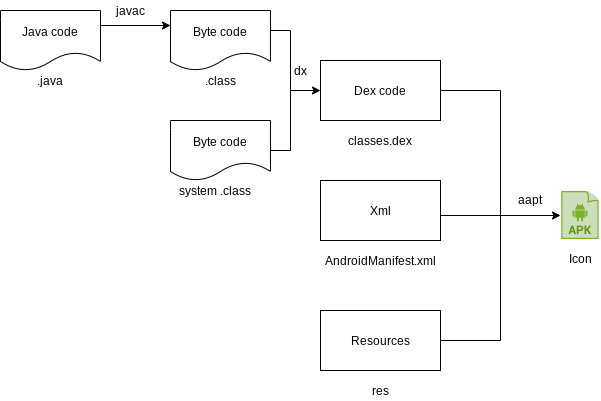
\includegraphics[width=0.9\textwidth]{figures/apk_structure}
\caption[Struttura di un file APK o Android Package]{Struttura di un file APK o Android Package
\label{fig:apk_structure}}
\end{figure}

\newpage

\section{Novità introdotte in ART}
\label{sec:nov_art}

Le novità introdotte con l'\emph{\gls{artg}} non si limitano al metodo di compilazione, ma in particolare:
\begin{itemize}
    \item \emph{Miglioramenti al \gls{garbcollg}\glsfirstoccur}: prima di \emph{ART} il \emph{\gls{garbcollg}} poteva provocare scarse performance alle applicazioni, compromettendo la loro reattività oltre a comportare altri problemi. Da \emph{Android Oreo 8.0} il \emph{\gls{garbcollg}} viene eseguito parallelamente, in modo da compromettere meno le performance e il suo tempo di esecuzione è stato ridotto. Oltre a questo è stato compattato riducendo la memoria utilizzata a runtime;
    
    \item \emph{Ottimizzazione dei cicli}: da \emph{Android Oreo 8.0} i loop vengono semplicificati durante la compilazione. In particolare vengono eliminate le variabili di induzione e sostituite con delle espressioni in forma chiusa;
    
    \item \emph{Devirtualizzazione di metodi}: da \emph{Android Oreo 8.0} viene utilizzata la \emph{\gls{chag}}\glsfirstoccurspace per devirtualizzare le chiamate virtuali in chiamate dirette, vista la complessità della ricerca nella \emph{vtable\_} per le chiamate virtuali;
    
    \item \emph{Inline cache}: da \emph{Android Oreo 8.0} viene introdotta la \emph{inline cache} nei file \emph{.oat} per ottimizzare le chiamate. Inoltre viene utilizzata per aggiungere informazioni utili a runtime;
    
    \item \emph{Dexlayout}: è una libreria introdotta per riordinare il codice \emph{\gls{dexfileg}} in modo da raggruppare le parti utilizzate più spesso per garantire un accesso più veloce in memoria;
    
    \item \emph{Metodi nativi più veloci}: da \emph{Android Nougat 7.0} sono disponibili chiamate più veloci alla \emph{Java Native Interface} usando le notazioni \emph{@FastNative} e \emph{@CriticalNative};
    
    \item \emph{Miglioramenti per il debugging e lo sviluppo}: vengono aggiunte più opzioni per il debugging e aumentati i dettagli diagnostici in caso di errori a runtime. \emph{\gls{artg}} fornisce appunto lo \emph{\gls{stacktraceg}}\glsfirstoccurspace non solo sul codice \emph{Java} ma anche sul codice nativo, inoltre le informazioni ritornate in caso di eccezione sono più accurate. Con le nuove opzioni per il debugging principalmente è possibile vedere il numero di occorrenze di una determinata classe a runtime, filtrare gli eventi per un'istanza precisa, visualizzare il valore restituito dai metodi ed impostare dei watchpoint. Viene aggiornato il \emph{Traceview}, in modo da evitare che possa compromettere le prestazione a runtime, come faceva in \emph{Dalvik} per colpa della compilazione a tempo di esecuzione. \emph{\gls{artg}}  fornisce un \emph{Traceview} dedicato per superare questi limiti e per fornire informazioni più dettagliate sull'esecuzione a runtime.
\end{itemize}

\section{Compilazione ibrida}
\label{sec:art_com_ibrid}

La compilazione ibrida di \emph{ART} combina gli aspetti positivi della compilazione \emph{JiT} con gli aspetti positivi della compilazione \emph{AoT}.

In particolare la soluzione adottata fino ad \emph{Android KitKat 4.4} contribuiva a:
\begin{itemize}
    \item Installazione più veloce;
    \item Poca memoria secondaria richiesta per l'installazione;
    \item Consumo eccessivo di batteria;
    \item Compilazione a tempo di esecuzione.
\end{itemize}
Mentre la soluzione \emph{AoT}:
\begin{itemize}
    \item Installazione lenta;
    \item Memoria secondaria richiesta per l'installazione eccessiva;
    \item Alte performance a tempo di esecuzione;
    \item Basso consumo di batteria.
\end{itemize}

La compilazione ibrida si basa sul fatto che l'utente non utilizza mai tutte le funzionalità di un'applicazione.
Il \emph{JiT runtime}, il compilatore JiT, si occupa di calcolare il livello di utilizzo di ogni metodo dell'applicazione e decidere quali metodi compilare a runtime e quali compilare precedentemente. Il field utilizzato per misurare il livello di utilizzo di un metodo è l'\emph{hotness\_count}, che verrà citato nelle prossime sezioni e nel capitolo \ref{chap:analisi_art}, \nameref{chap:analisi_art}. 

Il \emph{JiT compiler}, una volta che viene interpretato un metodo, crea un \emph{profile file}, che contiene informazioni sul tipo di compilazione deciso del metodo da parte del \emph{JiT compiler}. Appunto, se l'\emph{hotness\_count} supera una certa soglia, il metodo viene classificato "hot" e verrà compilato per essere eseguito successivamente senza bisogno di interpretarlo. Il servizio \emph{BackgroundDexOptService} si occupa di compilare e salvare in una \emph{JiT cache} i metodi "hot" segnalati nel \emph{Profile File} dell'applicazione in questione, durante la ricarica o periodi di inattività dello smartphone.

Il compilatore di Android che permette di precompilare il \emph{bytecode Java} è il \emph{dex2oat}, che salva i risultati ottenuti in un file \emph{.oat}.
Per precaricare le classi di \emph{Java} usate a runtime, viene creato un file \emph{boot.art} dal \emph{dex2oat}. Il file \emph{boot.art} contiene le classi pre-inizializzate e gli oggetti dal framework di \emph{Android}. In questo modo le applicazioni possono chiamare le \emph{\gls{apig}} del framework di \emph{Android} tramite \emph{boot.art}.



L'esecuzione di un'applicazione viene descritta in Fig. \ref{fig:jit_workflow}, e in particolare:

\begin{itemize} 
    \item l'utente sta eseguendo l'applicazione e viene richiesto l'utilizzo di un metodo contenuto nel \emph{\gls{bytejavag}} (\emph{\gls{dexfileg}});
    \item se il metodo è compilato \emph{AoT} allora viene eseguito direttamente il codice nativo contenuto nel file \emph{.oat}, altrimenti se il metodo è compilato \emph{JiT} precedentemente allora viene eseguito il codice nativo dal \emph{JiT code cache};
    \item se il metodo non è compilato, allora viene interpretato, e vengono aggiunte informazioni sul    \emph{Profile File} dell'applicazione riguardanti il metodo;
    \item se il metodo non compilato ha un \emph{hotness\_count} tale da definirlo "hot", allora il metodo viene compilato;
    \item una volta compilato, se è disponibile spazio sufficiente nella memoria il metodo viene salvato nel \emph{JiT code cache}.
\end{itemize}


\newpage


\begin{figure} [H]
\center
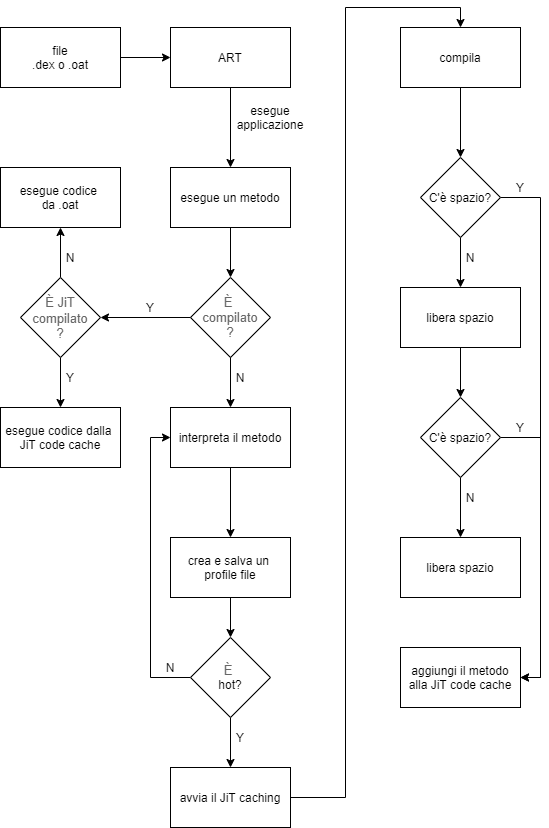
\includegraphics[width=0.9\textwidth]{figures/jit-workflow}
\caption[Android Runtime Just in Time Workflow]{Android ART JiT workflow
\label{fig:jit_workflow}}
\end{figure}


\section{Mirroring delle classi e metodi Java}




\emph{\gls{artg}} usa delle specifiche classi \texttt{C/C++} per il mirroring delle classi e dei metodi di Java. 
Il mirroring delle classi Java avviene tramite la classe \emph{Class}\footnote{android10-release/runtime/mirror/class.h} a basso livello, i cui puntatori vengono rappresentati nello Snippet \ref{lst:class}.

\begin{lstlisting}[language = C , frame = trBL , firstnumber = 1 , escapeinside={(*@}{@*)}, label={lst:class}, caption={Classe nativa Class},captionpos=b]
class MANAGED Class final : public Object {
  [..]
  HeapReference<ClassLoader> class_loader_;
  HeapReference<Class> component_type_;
  HeapReference<DexCache> dex_cache_;
  HeapReference<ClassExt> ext_data_;
  HeapReference<IfTable> iftable_;
  HeapReference<String> name_;
  HeapReference<Class> super_class_;
  HeapReference<PointerArray> vtable_;
  [..]
}
\end{lstlisting}

Attraverso delle \emph{HeapReference} la classe \emph{Class} contiene i riferimenti alle informazioni di una classe \emph{Java}, permettendo la sua esecuzione. I ruoli dei vari riferimenti si riassumono in:

\begin{itemize}
    \item \emph{class\_loader\_}: puntatore al \emph{\gls{classloaderg}}\glsfirstoccur;
    \item \emph{component\_type\_}: definisce il tipo dell'oggetto;
    \item \emph{dex\_cache\_}: puntatore ai metodi in cache;
    \item \emph{ext\_data\_}: data di classi esterne;
    \item \emph{iftable\_}: contiene i puntatori ai metodi interfaccia;
    \item \emph{name\_}: nome della classe;
    \item \emph{super\_class\_}: puntatore alla superclasse;
    \item \emph{vtable\_}: array di \emph{\gls{artmethodg}*} contenente i metodi virtuali.
\end{itemize}

\emph{Class} infine implementa tutti i metodi e i campi necessari per la gestione di una classe \emph{Java}.

\newpage

Il mirroring dei metodi in Java avviene tramite la classe \emph{ArtMethod}\footnote{android10-release/runtime/art\_method.h} a basso livello, i cui \emph{fields} sono rappresentati nello Snippet \ref{lst:artmethod}.


\begin{lstlisting}[language = C , frame = trBL , firstnumber = 1 , escapeinside={(*@}{@*)},
label={lst:artmethod}, caption={Classe nativa ArtMethod},captionpos=b]]
class ArtMethod final {
[..]
protected:
  GcRoot<mirror::Class> declaring_class_;
  std::atomic<std::uint32_t> access_flags_;
  uint32_t dex_code_item_offset_;
  uint32_t dex_method_index_;
  uint16_t method_index_;
  union {
    uint16_t hotness_count_;
    uint16_t imt_index_;
  };
  struct PtrSizedFields {
    void* data_;
    void* entry_point_from_quick_compiled_code_;
  } ptr_sized_fields_;
[..]
}
\end{lstlisting}

I ruoli dei \emph{field} contenuti nella classe \emph{\gls{artmethodg}} si riassumono in:

\begin{itemize}
    \item \emph{declaring\_class\_}: la classe a cui appartiene il metodo;
    \item \emph{access\_flags\_}: le keyword associate al metodo, come public, protected o private;
    \item \emph{dex\_code\_item\_offset\_}: l'offset del metodo all'interno del \emph{\gls{bytejavag}};
    \item \emph{dex\_method\_index\_}: index del metodo all'interno del \emph{\gls{bytejavag}};
    \item \emph{method\_index\_}: index del metodo. Per i metodi statici/diretti l'index è contenuto nell'array \emph{directMethods} mentre per i metodi virtuali nell'array \emph{vtable} e per i metodi interfaccia nell'array \emph{iftable};
    \item \emph{hotness\_count\_}: "hotness" del metodo, utilizzato per il \emph{JiT code caching}, come spiegato nella sezione \ref{sec:art_com_ibrid};
    \item \emph{int\_index\_}: specifica se il metodo è \emph{JiT cached};
    \item \emph{data\_}: in base al tipo di metodo ha diversi significati: può indicare un metodo nativo con un puntatore alla funzione JNI, un metodo astratto o di interfaccia, un proxy method oppure altri metodi;
    \item \emph{entry\_point\_from\_quick\_compiled\_code\_}: punta a un entry point nel caso il metodo sia stato compilato AoT.
\end{itemize}

I \emph{field} sopra descritti sono specifici per \emph{Android 10}, e nelle versioni più datate potrebbero cambiare notevolmente. Lo studio oggettivo dei valori dei suddetti \emph{field} viene descritto nel capitolo \ref{chap:analisi_art}.

\emph{\gls{artmethodg}} infine implementa tutti i metodi necessari alla gestione di un metodo \emph{Java}.

